\documentclass[11pt]{article}
\usepackage[utf8]{inputenc}

\title{ArcPy - module data access}
\author{Clément Delgrange}
\date{Avril 2018}

% Modules generaux
\usepackage[T1]{fontenc}
\usepackage[francais]{babel} % prise en charge du francais
\usepackage[table]{xcolor} % tableaux
\usepackage{graphicx} % images
\usepackage{float}
\usepackage[font=small]{caption}
\usepackage{enumitem}

% Marges
\usepackage[left=2cm,right=2cm,top=2cm,bottom=2cm]{geometry}

% Personnalisation des titres
\usepackage{titlesec}
\titlespacing{\section}{0em}{4em}{1em}
\titlespacing{\subsection}{0em}{2em}{0em}
\titlespacing{\subsubsection}{0em}{0.5em}{0em}

% Mise en page
\setlength{\parskip}{1.2em}
\renewcommand{\floatpagefraction}{1}

% Couleurs personnalisées
\usepackage{color}
\definecolor{lightgray}{gray}{0.98}
\definecolor{gray}{rgb}{0.6, 0.6, 0.65}
\definecolor{green}{rgb}{0.133, 0.545, 0.133}
\definecolor{blue}{rgb}{0, 0, 1}
\definecolor{red}{rgb}{0.6, 0.1, 0.1}

% Liens hypertextes
\usepackage{hyperref}
\hypersetup{
	colorlinks=true,
	breaklinks=true,
	urlcolor=blue,
	linkcolor=blue,
	pdfborder=000,
	pdftex=true
}

% Mise en forme des codes python
\usepackage{listingsutf8}
\lstset{
	language=python,
	inputencoding=utf8/latin1,
	extendedchars=true,
	keywordstyle=\bfseries\ttfamily\color{blue},
	identifierstyle=\ttfamily,
	commentstyle=\color{gray},
	stringstyle=\ttfamily\color{green},
	showstringspaces=false,
	basicstyle=\footnotesize\ttfamily,
	tabsize=2,
	breaklines=true,
	extendedchars=true,
	xleftmargin=1cm,
	xrightmargin=1cm,
	backgroundcolor=\color{lightgray},
	literate=%
		{é}{{\'{e}}}1
		{è}{{\`{e}}}1
		{ê}{{\^{e}}}1
		{ë}{{\¨{e}}}1
		{û}{{\^{u}}}1
		{ù}{{\`{u}}}1
		{â}{{\^{a}}}1
		{à}{{\`{a}}}1
		{î}{{\^{i}}}1
		{ô}{{\^{o}}}1
		{ç}{{\c{c}}}1
}

% Commandes personnalisées
\newcommand{\bslash}{\texttt{\symbol{92}}}
\newcommand{\action}{$\Rightarrow$ }
\newcommand{\reponse}{
	\begin{tabbing}
	\hspace{2cm}\=\kill
	Réponse \> ............................................................................................ \\
 	\> ............................................................................................
	\end{tabbing}
}

\newenvironment{note}{%
	\begin{tabular}[t t]{c c}
		
\includegraphics{img/tips.png}
		 &
		\begin{minipage}[c]{0.9\linewidth}
			\begin{sffamily}
}{%
			\end{sffamily}
		\end{minipage}
	\end{tabular}
}

\newenvironment{objectifs}{
  \hrule
	\begin{minipage}{0.9\textwidth}
		\vspace{1em}
		\begin{tabular}[t t]{c c}
			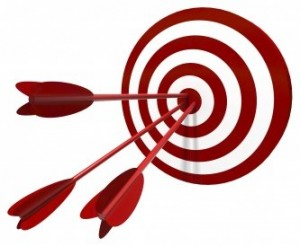
\includegraphics[width=0.1\linewidth]{img/goals.jpg} &
			\begin{minipage}[c]{0.8\linewidth}
				\hspace{2em}\textbf{\large{Objectifs :}} \\
}{
			\end{minipage}
		\end{tabular}
		\vspace{1em}
	\end{minipage}
	\hrule
}

\newcommand{\code}[1]{\lstinline{#1}}

\newenvironment{python}{%
	\begin{lstlisting}
}{%
	\end{lstlisting}
}

% Entetes et pieds de page
\usepackage{fancyhdr}
\pagestyle{fancy}
\fancyhf{}
\renewcommand{\headrulewidth}{0pt}
\makeatletter
\fancyfoot[L]{\@author}
\fancyfoot[C]{-\thepage-}
\fancyfoot[R]{\@title}
\makeatother
\renewcommand{\footrulewidth}{0.5pt}


%%%%%%%%%%%%
%%% Document
%%%%%%%%%%%%
\begin{document}
\parindent=0cm


\begin{titlepage}
\makeatletter
	\begin{sffamily}
		\begin{flushleft}
			% 
\includegraphics{img/logos/ign-logo-ensg.jpg}\\[1.5cm]
		\end{flushleft}
		\begin{flushright}
			% pour mettre une image en haut à droite
		\end{flushright}

		\vspace{4cm}

		\begin{center}
			\hrule
				\vspace{1em}
				{\small \textit{Programmation SIG}}\\
				\vspace{0.5cm}
				{\huge\bfseries \@title}
				\vspace{1cm}
			\hrule

			\vspace{3cm}
			%\includegraphics[width=400px]{images/logo_python.png}
			\begin{objectifs}
			\begin{itemize}
				\item enchaîner des géotraitements pour effectuer des opérations complexes
				\item découvrir le module d'accès aux données de la bibliothèque Arcpy et en particulier :
				\begin{itemize}
					\item savoir utiliser les curseurs
					\item être capable de manipuler les géométries
				\end{itemize}
			\end{itemize}
			\end{objectifs}
			\vspace{4cm}

			\large \textit{\@author}\\
			\small \textit{\@date}
		\end{center}
	\end{sffamily}
\makeatother
\end{titlepage}



\section{Traitement d'une couche de végétation}

\subsection{Énoncé du problème}

Nous nous intéressons à la répartition des arbres sur un territoire. Des saisies manuelles ou semi-automatiques ont été permis de localiser la position (emprise du houppier) de chacun des arbres de la zone d'étude. On nous demande, en partant de cette saisie, d'identifier quatre types de situation :
\begin{itemize}
	\item l'arbre est dit \textit{isolé} : il se situe à une distance suffisante de tous les autres arbres;
	\item un groupe d'arbres forme un ensemble d'\textit{arbres alignés} : les arbres sont dissociables mais sont suffisamment proche de leurs voisins et l'ensemble des arbres forme un ligne clairement identifiable;
	\item un groupe d'arbres forme un \textit{bosquet} : petit groupe d'arbres non dissociables de leur(s) voisin(s);
	\item un groupe d'arbres forme une \textit{zone arborée} : gros groupe d'arbres non dissociables de leurs voisins.
\end{itemize}

\subsubsection{Fichier final}

Toute la végétation devra être rendue dans un seul shapefile qui comportera les attributs listés dans le tableau ci-dessous.

\begin{table}[H]
\centering
\begin{tabular}{|l|p{5cm}|l|l|}
\hline
\textbf{Nom}	& \textbf{Description}		& \textbf{Type}		& \textbf{Restrictions} \\
\hline
\textbf{TYPE}			& Type de végétation		& Caractère(30)		& \begin{tabular}{l}Obligatoire\\ Liste de valeurs :\\ 1-Arbre isolé\\ 2-Arbres alignés\\ 3-Bosquet\\ 4-Zone arborée\end{tabular} \\
\hline
\textbf{SURFACE}			& Surface calculée			& Décimal(10,2)		& \begin{tabular}{l}Obligatoire\\ Unité $m^2$\end{tabular} \\
\hline
\textbf{LARGEUR}			& Diamètre ou largeur de l'objet à l'endroit le plus large
											& Décimal(4,1)		& \begin{tabular}{l}Obligatoire si type=\{1, 2\}\\ Unité m\end{tabular} \\
\hline
\textbf{LONGUEUR}		& Longueur de l'objet		& Décimal(4,1)		& Obligatoire si type=\{2\} \\
\hline
\textbf{NB\_ARBRE}		& Nombre d'arbres			& Entier court		& Obligatoire \\
\hline
\textbf{REMARQUE}		& Remarques éventuelles		& Caractère(200)	& Optionnel \\
\hline
\end{tabular}
\end{table}


\subsubsection{Spécifications de saisie}

Les spécifications de saisie pour chacun de ces objets sont :
\begin{itemize}[label=$\bullet$]
	\item \underline{\textbf{Arbres alignés}}
	\begin{itemize}
		\item Spécification : arbres dont les houppiers ne se touchent pas et dont la distance entre les houppiers est inférieure à 3m. L'angle entre deux arbres consécutifs de l'alignement doit être compris entre $150$ et $210^{\circ}$.
		\item Géométrie : buffer construit sur l'axe passant par le centre de tout les arbres de l'alignement et de largeur égale à le moyenne des largeur des arbres.
		\item Règle de remplissage des attributs : \\
		LARGEUR = largeur du plus gros arbre de l'alignement\\
		LONGUEUR = longueur totale tronc à tronc de l'alignement.
	\end{itemize}
	\item \underline{\textbf{Arbres isolé}}
	\begin{itemize}
		\item Spécification : arbre dont le houppier ne touche aucun autre houppier et qui ne fait pas parti d'un alignement.
		\item Géométrie : houppier de l'arbre.
		\item Règle de remplissage des attributs : \\
		NB\_ARBRE = 1\\
		LARGEUR = diamètre de l'arbre.
	\end{itemize}
	\item \underline{\textbf{Bosquet}}
	\begin{itemize}
		\item Spécification : ensemble constitué de 2 à 10 arbres (inclus) dont les houppiers se touchent ou se chevauchent.
		\item Géométrie : la surface du bosquet est celle de l'ensemble des houppiers des arbres qui le constitue en ayant pris soin de combler les trous entre les arbres s'il y en a.
		\item Règle de remplissage des attributs : - \\
	\end{itemize}
	\item \underline{\textbf{Zone arborée}}
	\begin{itemize}
		\item spécification : ensemble constitué de plus de 10 arbres dont les houppiers se touchent ou se chevauchent. La surface de la zone arborée est constitué de l'ensemble des houppiers des arbres qui la constitue en "lissant" les bords et en supprimant éventuellement les trous.
		\item Règle de remplissage des attributs : - \\
	\end{itemize}
\end{itemize}

\subsubsection{Exemples}

\begin{figure}[H]
	\center 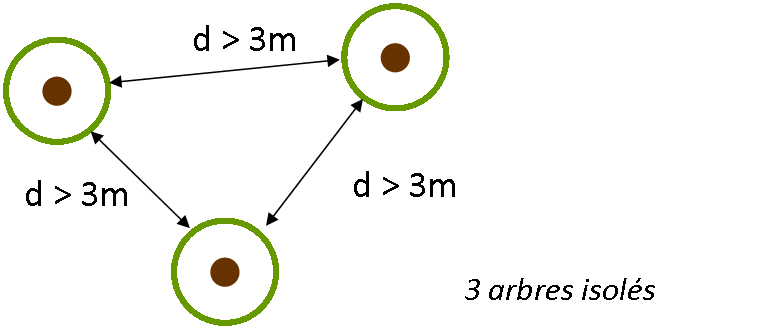
\includegraphics[width=0.45\textwidth]{img/td_arcpy_da/arbres_isoles.png}\\
\end{figure}

\vspace{2em}

\begin{figure}[H]
	\center 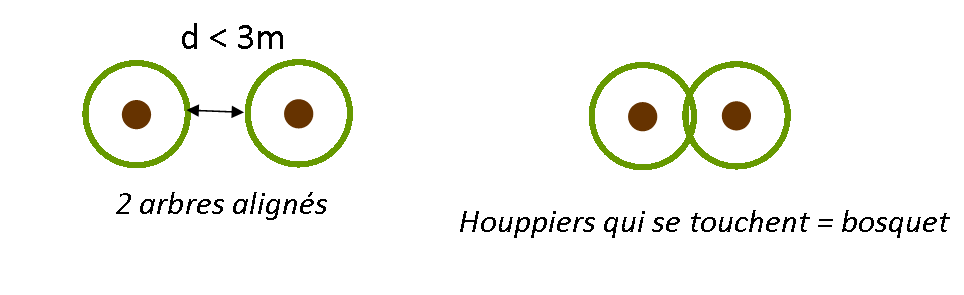
\includegraphics[width=0.6\textwidth]{img/td_arcpy_da/arbres_alignes_bosquet.png}\\
\end{figure}

\vspace{2em}

\begin{figure}[H]
	\center 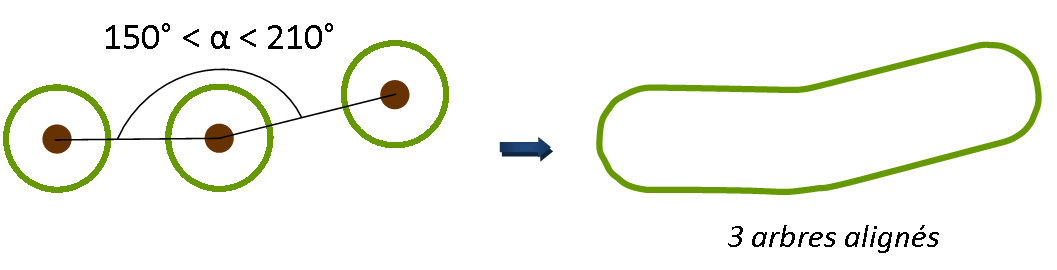
\includegraphics[width=0.7\textwidth]{img/td_arcpy_da/arbres_alignes.png}\\
\end{figure}

\vspace{2em}

\begin{figure}[H]
	\center 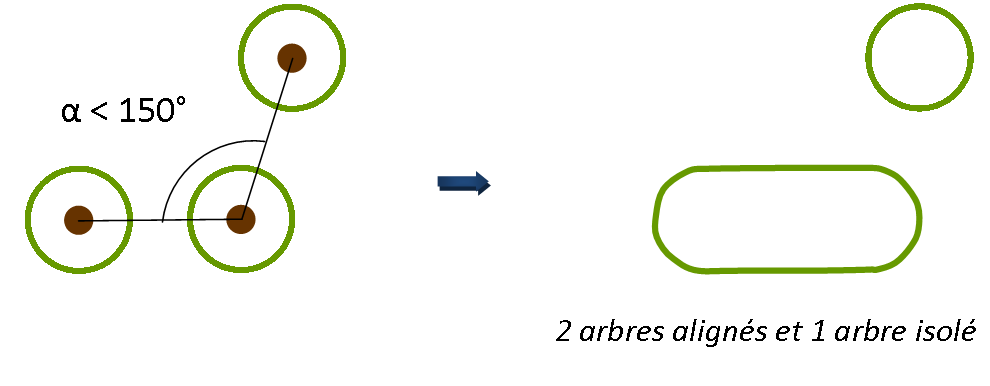
\includegraphics[width=0.7\textwidth]{img/td_arcpy_da/arbres_alignes_isole.png}\\
\end{figure}

\vspace{2em}

\begin{figure}[H]
	\center 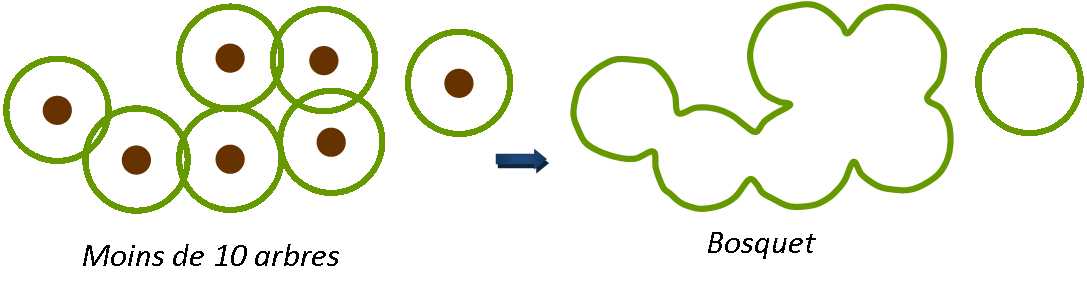
\includegraphics[width=0.85\textwidth]{img/td_arcpy_da/bosquet.png}\\
\end{figure}

\vspace{2em}

\begin{figure}[H]
	\center 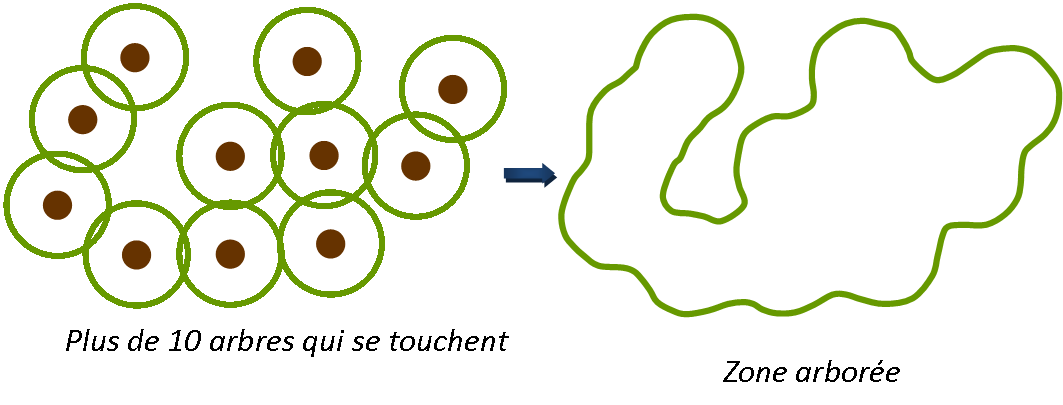
\includegraphics[width=0.8\textwidth]{img/td_arcpy_da/zone_arboree.png}\\
\end{figure}


\subsection{Travail demandé}

\action Écrivez un (ou plusieurs) script(s) Python, basé(s) la librairie ArcPy, permettant d'effectuer les transformations demandées sur une couche de végétation qui vous est fournie.

Vous utiliserez le mode de diffusion qui vous semble le plus approprié.


\action Si vous avez un script fonctionnel, faites le tourner sur le jeu test et analysez le résultat. Proposez des évolutions des spécifications pour mieux rendre compte de certaines réalités.


\end{document}
